\documentclass{article}
\usepackage{graphicx}
\usepackage{tikz}
\usepackage{pgfplots}
\usepackage{circuitikz}
\usepackage[spanish]{babel}
\usepackage{fancyhdr}
\usepackage[bottom, norule]{footmisc}
\usepackage{multicol}
\usepackage{sectsty}
\usepackage{amsmath}
\usepackage{hyperref}
\usepackage[square,numbers,sort&compress]{natbib}
\usepackage[hypcap=false]{caption}

\bibliographystyle{apsrev4-2}

\title{Informe Laboratorio 03}
\date{Septiembre 2025}

\pgfplotsset{compat=1.18}
\pgfplotsset{width=6cm}

\begin{document}

\fancyfoot[C]{}
\fancyhead{}

%-------------------------------------------
% ENCABEZADO CON LOGOS
%-------------------------------------------
\begin{tikzpicture}[remember picture, overlay]
\node[anchor=north west, xshift=2.6cm, yshift=-0.5cm] at (current page.north west)
{
\includegraphics[width=3.5cm]{img/marcaderecha.png}};
\node[anchor=north east, xshift=-2.6cm, yshift=-1cm] at (current page.north east)
{
\includegraphics[width=4cm]{img/logo-cfm.png}};
\end{tikzpicture}

\begin{center}
\large Laboratorio I \\[0.3cm]
{\scshape\Huge Bobina de Helmholtz y permeabilidad magnética \par}
\vspace{0.5cm}
{\large Nombres: Bruno Bustos, Darío Ferrada, Camilo Jordán, Catalina Zamorano}\\[0.3cm]
\ttfamily Universidad de Concepción, Facultad de Ciencias Físicas y Matemáticas
\end{center}

\vspace{1cm}

%-------------------------------------------
\begin{abstract}
En este informe se utiliza una bobina de Helmholtz para medir experimentalmente la
permeabilidad magnética del aire. Se desarrolla el modelo teórico del campo magnético
generado por la bobina y se comparan los resultados experimentales con el valor teórico
esperado, analizando las principales fuentes de error y su impacto en la medición.
\end{abstract}

%-------------------------------------------
\section*{Introducción}

En problemas de electromagnetismo se emplean diversas expresiones para calcular campos
magnéticos; sin embargo, resulta fundamental comprender el significado físico de las
constantes que aparecen en dichas expresiones. En particular, la permeabilidad magnética
caracteriza la capacidad de un material para permitir la propagación de un campo magnético.

En este trabajo se determina experimentalmente la permeabilidad magnética del aire,
aproximada por la permeabilidad del vacío $\mu_0$, utilizando una bobina de Helmholtz,
comparando el resultado obtenido con el valor teórico aceptado.

\newpage

%-------------------------------------------
\section*{Modelo teórico}

El campo magnético generado por una espira circular de radio $R$ que transporta una corriente
$I$, evaluado sobre su eje a una distancia $x$ del centro, está dado por \cite{Griffiths}:

\begin{equation}
B(x) = \frac{\mu_0 I R^2}{2\left(R^2 + x^2\right)^{3/2}}.
\end{equation}

En una configuración de Helmholtz, dos bobinas idénticas se disponen de forma coaxial y se
separan una distancia igual a su radio $R$. Tomando el origen en el punto medio entre ambas,
estas se ubican en $x=\pm R/2$. El campo total en el centro corresponde a la suma de los
campos generados por cada bobina:

\begin{equation}
B_{\text{total}} = 2 B\left(\frac{R}{2}\right).
\end{equation}

Evaluando la expresión anterior:

\begin{align}
B\left(\frac{R}{2}\right)
&= \frac{\mu_0 I R^2}{2\left(R^2 + \frac{R^2}{4}\right)^{3/2}} \\
&= \frac{1}{2}\,\mu_0\,\frac{I}{R}\left(\frac{4}{5}\right)^{3/2}.
\end{align}

Por lo tanto, el campo magnético total generado por una bobina de Helmholtz en su centro es
\cite{bobinaHz}:

\begin{equation}
B = \mu_0\,\frac{N I}{R}\left(\frac{4}{5}\right)^{3/2}.
\end{equation}

Esta expresión permite identificar una relación lineal entre el campo magnético y la
corriente:

\begin{equation}
B = \alpha I,
\qquad
\alpha = \mu_0 \frac{N}{R}\left(\frac{4}{5}\right)^{3/2}.
\label{eq:alpha}
\end{equation}

%-------------------------------------------
\section*{Materiales}

\begin{itemize}
\item Bobina de Helmholtz
\item Fuente de alimentación DC
\item Multímetro
\item Magnetómetro
\item Cables de conexión
\end{itemize}

%-------------------------------------------
\section*{Montaje experimental}

Las bobinas utilizadas poseen $N=77$ espiras cada una y se conectan en paralelo, presentando
una resistencia total del sistema $R_t = 0.8\,\Omega$. Debido a esta configuración, la
corriente total suministrada por la fuente se divide en partes iguales, por lo que la
corriente efectiva en cada bobina corresponde a $I = I_{\text{total}}/2$.

El radio de las bobinas es $R = 0.20\,\text{m}$ y el magnetómetro se posiciona en el centro
geométrico del sistema, tal como se muestra en la Figura~\ref{fig:bobina}.

\begin{center}
\captionsetup{type=figure}
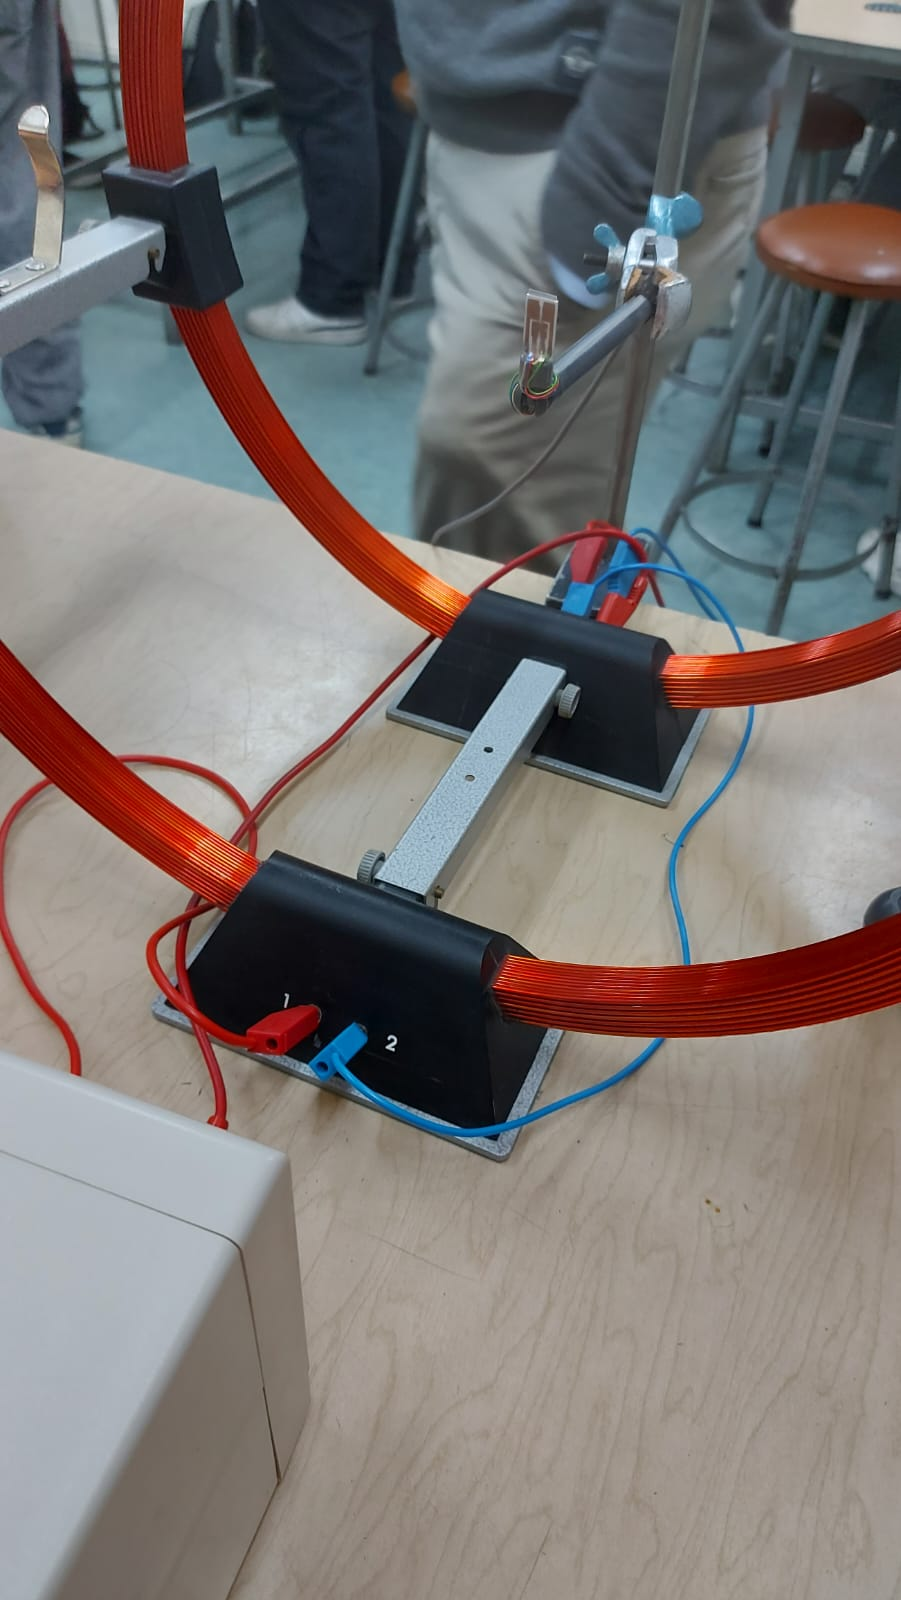
\includegraphics[width=0.5\columnwidth]{img/bobina.jpg}
\caption{Bobina en configuración de Helmholtz.}
\label{fig:bobina}
\end{center}

\newpage
%-------------------------------------------
\section*{Resultados experimentales}

A partir de las mediciones de voltaje se obtuvo la corriente por bobina utilizando la ley de
Ohm. El campo magnético fue medido directamente con el magnetómetro. Los datos obtenidos se
presentan en la Tabla \ref{tab:datos}.

\begin{center}
\small
\centering
\begin{tabular}{|c|c|c|c|}
\hline
\textbf{Vol V} & \textbf{I Total A} & \textbf{I Bobina A} & \textbf{B mT} \\
\hline
0.115 & 0.144 & 0.072 & 0.0200 \\ \hline
0.230 & 0.288 & 0.144 & 0.0450 \\ \hline
0.340 & 0.425 & 0.213 & 0.0615 \\ \hline
0.461 & 0.576 & 0.288 & 0.0750 \\ \hline
0.569 & 0.711 & 0.356 & 0.1000 \\ \hline
0.674 & 0.843 & 0.422 & 0.1150 \\ \hline
0.787 & 0.984 & 0.492 & 0.1250 \\ \hline
0.885 & 1.106 & 0.553 & 0.1500 \\ \hline
1.008 & 1.260 & 0.630 & 0.1600 \\ \hline
1.109 & 1.386 & 0.693 & 0.1800 \\ \hline
1.222 & 1.527 & 0.764 & 0.1950 \\ \hline
1.325 & 1.656 & 0.828 & 0.2150 \\ \hline
1.435 & 1.794 & 0.897 & 0.2250 \\ \hline
1.550 & 1.938 & 0.969 & 0.2500 \\ \hline
1.659 & 2.074 & 1.037 & 0.2650 \\ \hline
1.774 & 2.218 & 1.109 & 0.2850 \\ \hline
1.864 & 2.330 & 1.165 & 0.3000 \\ \hline
1.984 & 2.480 & 1.240 & 0.3150 \\ \hline
2.097 & 2.621 & 1.311 & 0.3350 \\ \hline
2.203 & 2.754 & 1.377 & 0.3500 \\ \hline
2.320 & 2.900 & 1.450 & 0.3650 \\ \hline
2.425 & 3.031 & 1.516 & 0.3850 \\ \hline
2.558 & 3.198 & 1.599 & 0.4000 \\ \hline
2.650 & 3.313 & 1.657 & 0.4150 \\ \hline
2.750 & 3.438 & 1.719 & 0.4300 \\ \hline
2.873 & 3.591 & 1.796 & 0.4500 \\ \hline
2.990 & 3.738 & 1.869 & 0.4700 \\ \hline
3.075 & 3.844 & 1.922 & 0.4850 \\ \hline
3.210 & 4.013 & 2.007 & 0.5000 \\ \hline
3.322 & 4.153 & 2.077 & 0.5250 \\ \hline
3.659 & 4.574 & 2.287 & 0.5750 \\ \hline
3.767 & 4.709 & 2.355 & 0.5850 \\ \hline
3.880 & 4.850 & 2.425 & 0.6000 \\ \hline
\end{tabular}

\captionof{table}{Voltaje, corriente y campo magnético. }
\label{tab:datos}
\end{center}

\newpage

Los errores instrumentales considerados fueron:

\begin{align}
\sigma_V &= 5\times 10^{-4}\,\text{V},\\
\sigma_I &= 5\times 10^{-4}\,\text{A},\\
\sigma_B &= 1\times 10^{-8}\,\text{T}.
\end{align}

%-------------------------------------------
\section*{Análisis y ajuste lineal}

En la Figura~\ref{fig:graficoBI} se presenta el gráfico del campo magnético $B$ en función de
la corriente $I$, junto con el ajuste lineal correspondiente. Los residuos del ajuste se
muestran en la Figura~\ref{fig:residuos}.

\begin{center}
\captionsetup{type=figure}
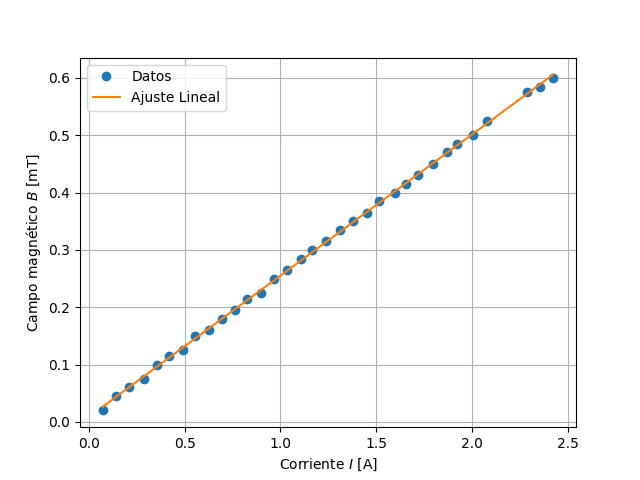
\includegraphics[width=0.5\columnwidth]{img/cosawena.png}
\caption{Campo magnético en función de la corriente junto con el ajuste lineal.}
\label{fig:graficoBI}
\end{center}

\begin{center}
\captionsetup{type=figure}
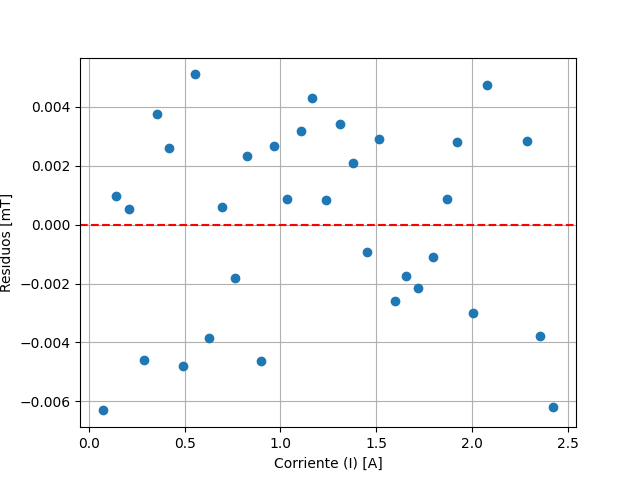
\includegraphics[width=0.5\columnwidth]{img/residuoslol.png}
\caption{Residuos del ajuste lineal $B$ vs $I$.}
\label{fig:residuos}
\end{center}

La pendiente obtenida del ajuste fue:

\begin{equation}
\alpha = (2.464 \pm 0.001)\times 10^{-4}\,\text{T/A}.
\end{equation}

%-------------------------------------------
\section*{Análisis de errores}

El error experimental se analizó a partir de la dispersión de los datos y del ajuste lineal
del campo magnético en función de la corriente. El modelo considerado es

\begin{equation}
B = \alpha I + B_0,
\end{equation}

donde $\alpha$ corresponde a la pendiente del ajuste y $B_0$ a la ordenada al origen.

La incertidumbre en la pendiente se obtuvo directamente de la matriz de covarianza del ajuste
lineal, resultando:

\begin{equation}
\alpha = (2.464 \pm 0.001)\times 10^{-4}\,\text{T/A}.
\end{equation}

Los residuos del ajuste, mostrados en la Figura~\ref{fig:residuos}, se distribuyen alrededor
de cero sin presentar tendencias sistemáticas, lo que indica que el modelo lineal describe
adecuadamente los datos experimentales. El error global del ajuste es del orden de $10^{-3}$
en unidades relativas.

La permeabilidad magnética experimental se obtiene a partir de la relación

\begin{equation}
\mu_0^{\text{exp}} = \alpha\,\frac{R}{N}\left(\frac{4}{5}\right)^{-3/2}.
\end{equation}

Suponiendo que las incertidumbres en $R$ y $N$ son despreciables frente a la de $\alpha$, la
propagación de errores queda dada por

\begin{equation}
\sigma_{\mu_0} = \mu_0^{\text{exp}} \frac{\sigma_\alpha}{\alpha}.
\end{equation}

De este modo, se obtiene:

\begin{equation}
\mu_0^{\text{exp}} = (8.95 \pm 0.06)\times 10^{-7}\,\text{H/m}.
\end{equation}

Pero si agregamos un posible error en el conteo de espiras, al calcular el valor de $\mu_0$
se obtiene la siguiente tabla de valores \ref{tab:mu_vs_N}.

\begin{center}
\small
\begin{tabular}{|c|c|}
\hline
\textbf{Número de espiras $N$} & $\boldsymbol{\mu_0^{\text{exp}}}$ \textbf{[H/m]} \\ \hline
75 & $9.19 \times 10^{-7}$ \\ \hline
76 & $9.07 \times 10^{-7}$ \\ \hline
77 & $8.95 \times 10^{-7}$ \\ \hline
78 & $8.83 \times 10^{-7}$ \\ \hline
79 & $8.72 \times 10^{-7}$ \\ \hline
\end{tabular}
\captionof{table}{Valor experimental de la permeabilidad magnética para distintos números de espiras, manteniendo fija la pendiente del ajuste.}
\label{tab:mu_vs_N}
\end{center}

%-------------------------------------------
\section*{Determinación de la permeabilidad magnética}

Utilizando la ecuación \eqref{eq:alpha}, se obtiene:

\begin{equation}
\mu_0^{\text{exp}} = \alpha\,\frac{R}{N}\left(\frac{4}{5}\right)^{-3/2}.
\end{equation}

Reemplazando valores experimentales:

\begin{equation}
\mu_0^{\text{exp}} = (8.95 \pm 0.06)\times 10^{-7}\,\text{H/m}.
\end{equation}

El valor teórico aceptado es $\mu_0 = 4\pi \times 10^{-7}\,\text{H/m}$ \cite{Griffiths}. El
error relativo se calcula como:

\begin{equation}
\varepsilon_r =
\left|
\frac{\mu_{\text{exp}} - \mu_{\text{teo}}}{\mu_{\text{teo}}}
\right| \times 100\% = 28.7\%.
\end{equation}

La discrepancia observada se atribuye principalmente a errores sistemáticos, tales como la
presencia del campo magnético terrestre, posibles desalineaciones del sensor y limitaciones
en la calibración del magnetómetro.

%-------------------------------------------
\section*{Predicción a futuro}

Dado que dentro del rango experimental la relación entre el campo magnético y la corriente
es lineal, el modelo ajustado

\begin{equation}
B = \alpha I
\end{equation}

puede utilizarse para predecir valores del campo magnético para corrientes no medidas. Para
una corriente futura $I_f$, el campo esperado está dado por

\begin{equation}
B_f = \alpha I_f.
\end{equation}

Esta predicción es válida mientras se mantengan las condiciones experimentales de medio
lineal, geometría constante y corrientes estacionarias. Desviaciones del modelo se
manifestarían como pérdida de linealidad o aumento sistemático de los residuos.

\begin{center}
\captionsetup{type=figure}
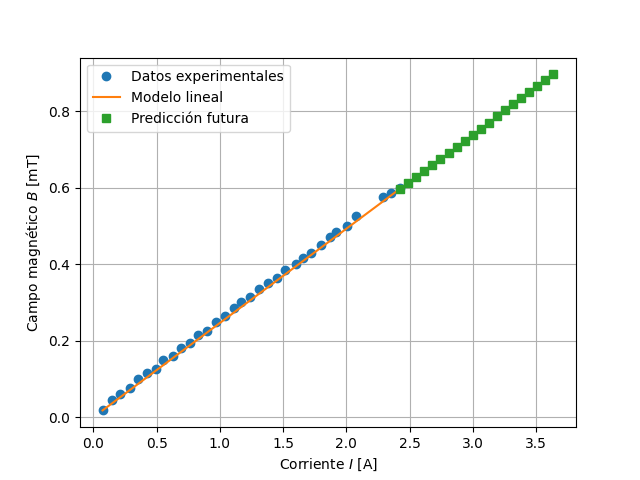
\includegraphics[width=0.5\columnwidth]{img/futuro.png}
\caption{Predicción del campo magnético para corrientes futuras.}
\label{fig:futuro}
\end{center}

%-------------------------------------------
\section*{Conclusiones}

Se determinó experimentalmente la permeabilidad magnética del aire utilizando una bobina de
Helmholtz, verificándose la relación lineal entre el campo magnético y la corriente. Aunque
el valor obtenido presenta una discrepancia del orden del 29\% respecto al valor teórico,
el comportamiento observado concuerda con el modelo esperado.

El experimento evidencia la sensibilidad de este tipo de mediciones a errores sistemáticos
y destaca la importancia de un adecuado control experimental.

\bibliography{referencias.bib}

\end{document}
